\documentclass[11pt]{article}
%\usepackage{amsfonts}
\usepackage{amsmath}
\usepackage{fancybox}%,times}
\usepackage{graphicx,psfrag,epsf}
%\usepackage{amsmath}
\usepackage{enumerate}
\usepackage{graphicx,psfrag}
\usepackage{multirow}
\usepackage{epsfig}
\usepackage[svgnames]{xcolor}
%\usepackage{rotating}
\usepackage{subfigure}
\usepackage{theorem}
\usepackage{natbib,psfrag}
\usepackage{tikz}
\usepackage{xcolor}
\usepackage{kotex}
\newcommand{\blind}{0}
\usepackage{graphicx}
\usepackage{listings}


%\documentclass[a4paper,12pt]{article}
\usepackage[utf8]{inputenc}

% Default fixed font does not support bold face
\DeclareFixedFont{\ttb}{T1}{txtt}{bx}{n}{12} % for bold
\DeclareFixedFont{\ttm}{T1}{txtt}{m}{n}{12}  % for normal

% Custom colors
\usepackage{color}
\definecolor{deepblue}{rgb}{0,0,0.5}
\definecolor{deepred}{rgb}{0.6,0,0}
\definecolor{deepgreen}{rgb}{0,0.5,0}

\usepackage{listings}
\DeclareGraphicsExtensions{.pdf,.png,.jpg}

\addtolength{\oddsidemargin}{-.75in}%
\addtolength{\evensidemargin}{-.75in}%
\addtolength{\textwidth}{1.5in}%
\addtolength{\textheight}{1.3in}%
%\addtolength{\topmargin}{-.6in}%
\addtolength{\topmargin}{-.8in}%

%\theoremstyle{break}
\newtheorem{The}{Theorem}
\newtheorem{Def}{Definition}
\newtheorem{Pro}{Proposition}
\newtheorem{Lem}{Lemma}
\newtheorem{Cor}{Corollary}
\newtheorem{asp}{Assumption}


\renewcommand{\thefootnote}{\arabic{footnote}}
%\renewcommand{\thefootnote}{\alph{footnote}}
%\renewcommand{\thefootnote}{\roman{footnote}}
%\renewcommand{\thefootnote}{\fnsymbol{footnote}}

\begin{document}
	
	
	%\bibliographystyle{natbib}
	
	\newcommand{\Ito}{$It\hat{o}$'$s~Lemma$}
	
	\newcommand\ind{\stackrel{\rm ind}{\sim}}
	\newcommand\iid{\stackrel{\rm iid}{\sim}}
	\renewcommand\c{\mathbf{c}}
	\newcommand\y{\mathbf{y}}
	\newcommand\z{\mathbf{z}}
	\renewcommand\P{\mathbf{P}}
	\newcommand\W{\mathbf{W}}
	\newcommand\X{\mathbf{X}}
	\newcommand\Y{\mathbf{Y}}
	\newcommand\Z{\mathbf{Z}}
	\newcommand\J{{\cal J}}
	\newcommand\B{{\cal B}}
	\newcommand\K{{\cal K}}
	\newcommand\N{{\rm N}}
	\newcommand\bs{\boldsymbol}
	\newcommand\bth{\bs\theta}
	\newcommand\bbe{\bs\beta}
	\renewcommand\*{^\star}
	\newcommand{\notimplies}{%
		\mathrel{{\ooalign{\hidewidth$\not\phantom{=}$\hidewidth\cr$\implies$}}}}
	
	\def\spacingset#1{\renewcommand{\baselinestretch}%
		{#1}\small\normalsize} \spacingset{1}
	
	
	%%%%%%%%%%%%%%%%%%%%%%%%%%%%%%%%%%%%%%%%%%%%%%%%%%%%%%%%%%%%%%%%%%%%%%%%%%%%%%
	
	\bigskip
	\bigskip
	\bigskip
	\begin{center}
		{\LARGE\bf 2019 Oct. 31 }
	\end{center}
	\begin{center}
		2018321084 Juyoung Ahn
	\end{center}
	\medskip
	
	%\begin{abstract}
	%\end{abstract}
	
	%\noindent%
	%{\it Key Words:}  AECM algorithm; Astrophysical data analysis;
	%ECME algorithm; Incompatible Gibbs sampler; Marginal data
	%augmentation; Multiple imputation; Spectral analysis
	
	\spacingset{1.45}
	\section{Gaussian 2 changing point model}
	\subsection{likelihood and prior}
	\begin{align*}
		\beta_t &\ind \begin{cases}
		N(\mu_1, \tau_1^{-1}) \;\; \text{for } t = 1,\dots,k\\
		N(\mu_2, \tau_2^{-1}) \;\; \text{for } t = k+1,\dots,T
		\end{cases}\\
	\end{align*}
	Where ,
	\begin{align*}
		\mu_1 &\sim N(0, b_1^{-1})\\
		\mu_2 &\sim N(0, b_2^{-1})\\
		\tau_1 &\sim Gamma(c_1, d_1)\\
		\tau_2 &\sim Gamma(c_2, d_2)\\
		k &\sim unif\{1,T\}
	\end{align*}
	Then,
	\begin{align*}
		p(\mu_1, \mu_2,\tau_1,\tau_2,k  | \boldsymbol{\beta})\propto& p(\boldsymbol{\beta} | \mu_1, \mu_2,\tau_1,\tau_2,k ) p(\mu_1) p(\mu_2) p(\tau_1)p(\tau_2)\\
		\propto& (\tau_1)^{\frac{k}{2}} \exp\left(-\frac{1}{2} \tau_1 \sum_{t=1}^{k}(\beta_t - \mu_1)^2\right)\\
		&\times (\tau_2)^{\frac{T-k}{2}} \exp\left(-\frac{1}{2} \tau_2 \sum_{t=k+1}^{T}(\beta_t - \mu_2)^2\right)\\
		&\times b_1^{\frac{1}{2}} \exp\left(-\frac{1}{2}b_1 \mu_1^2\right) \times b_2^{\frac{1}{2}} \exp\left(-\frac{1}{2}b_2 \mu_2^2\right)\\
		&\times \tau_1^{c_1-1} \exp(-d_1 \tau_1) \times \tau_2^{c_2-1} \exp(-d_2 \tau_2)\\
		&\times 1
	\end{align*}
	\subsection{Gibbs sampler}
	\begin{align*}
		\mu_1 | \mu_2,\tau_1,\tau_2,k,\boldsymbol{\beta} &\sim N\left((k \cdot \tau_1+b_1)^{-1}\tau_1\sum_{t=1}^{k}\beta_t ,(k \cdot \tau_1+b_1)^{-1}\right)\\
		\mu_2 | \mu_1,\tau_1,\tau_2,k,\boldsymbol{\beta} &\sim N\left(((T-k) \cdot \tau_2+b_2)^{-1}\tau_2\sum_{t=k+1}^{T}\beta_t ,((T-k) \cdot \tau_2+b_2)^{-1}\right)\\
		\tau_1 | \mu_1 ,\mu_2,\tau_2,k,\boldsymbol{\beta} & \sim Gamma\left(c_1 + \frac{k}{2}, \frac{1}{2} \sum_{t=1}^k (\beta_t - \mu_1)^2 +d_1\right)\\
		\tau_2 | \mu_1 ,\mu_2,\tau_1,k,\boldsymbol{\beta} & \sim Gamma\left(c_2 + \frac{T-k}{2}, \frac{1}{2} \sum_{t=k+1}^T (\beta_t - \mu_2)^2 +d_2\right)\\
		p(k | \mu_1,\mu_2,\tau_1,\tau_2,\boldsymbol{\beta}) & \propto \exp\left(\frac{1}{2} \sum_{t=1}^k \left[ \tau_2(\beta_t - \mu_2)^2 - \tau_1 (\beta_t - \mu_1)^2\right] + \frac{k}{2} \log(\tau_1/\tau_2)\right) = H(k)\\
		p(k | \mu_1,\mu_2,\tau_1,\tau_2,\boldsymbol{\beta}) &= \frac{H(k)}{\sum_{t=1}^T H(k)}
	\end{align*}
	\subsection{Variational Bayes}
	Let the variational distribution is
	\begin{align*}
		q_1^*(\mu_1) &\sim N(m_1,s_1)\\
		q_2^*(\mu_2) &\sim N(m_2,s_2)\\
		q_3^*(\tau_1) &\sim Gamma(\gamma_1,\eta_1)\\
		q_4^*(\tau_2) &\sim Gamma(\gamma_2,\eta_2)\\
		q_5^*(k) &\sim Categorical
	\end{align*}
		Then $E_{q_5^*}(k) = \sum_{t=1}^k k \cdot q_5^*(k)$, and 
	\begin{align*}
		q_{1^*}(\mu_1) \sim& N\left(\left[E_q^*[k] \frac{\gamma_1}{\eta_1}+b_1\right]^{-1}\frac{\gamma_1}{\eta_1}\sum_{t=1}^{E_q^*[k]}\beta_t ,\left(E_q^*[k]\frac{\gamma_1}{\eta_1}+b_1\right)^{-1}\right)\\
		q_{1^*}(\mu_2) \sim& N\left(\left  (T- [E_q^*[k]) \frac{\gamma_2}{\eta_2}+b_2\right]^{-1}\frac{\gamma_2}{\eta_2}\sum_{t=E_q^*[k]+1}^{T}\beta_t ,\left( (T-E_q^*[k])\frac{\gamma_2}{\eta_2}+b_2\right)^{-1}\right)\\
		q_{1^*}(\tau_1)  \sim& Gamma\left(c_1 + \frac{E_q^*[k]}{2}, \frac{1}{2} \sum_{t=1}^{E_q^*[k]} \left\{\beta_t^2 - 2\beta_t m_1 + m_1^2 + s_1 \right\} +d_1\right)\\
		q_{1^*}(\tau_2)  \sim& Gamma\left(c_2 + \frac{T - E_q^*[k]}{2}, \frac{1}{2} \sum_{t=E_q^*[k]+1}^{T} \left\{\beta_t^2 - 2\beta_t m_2 + m_2^2 + s_2 \right\} +d_2\right)\\
		q_{1^*}(\mu_1)  =& \frac{\mathcal{H}(k)}{\sum_{t=1}^T \mathcal{H}(k)}\\
		\log(\mathcal{H}(k))  =&\frac{1}{2} \sum_{t=1}^k \left[ \frac{\gamma_2}{\eta_2}(\beta_t^2 -2\beta_t m_2 + m_2^2 + s_2) - \frac{\gamma_1}{\eta_1}(\beta_t^2 -2\beta_t m_1 + m_1^2 + s_1)\right] \\ &+ \frac{k}{2} (-\log\eta_1 + \psi(\gamma_1) + \log\eta_2 - \psi(\gamma_2)))
	\end{align*}
	We can use
	\begin{align*}
	X \sim Gamma(\alpha,\beta)\\
	E[\log X] = -\log\beta +\psi(\alpha)
	\end{align*}
	where $\psi$ means digamma function
	Prior and initial value are
	
	\section{Simulation}
	Make simulation data from
	\begin{align*}
	\beta_t &\iid \begin{cases}
	N(1,1)\;\; t= 1, \dots ,30 \\
	N(0,1) \;\; t= 31, \dots ,100
	\end{cases}
	\end{align*}

	\begin{figure} [h]
		\centering
		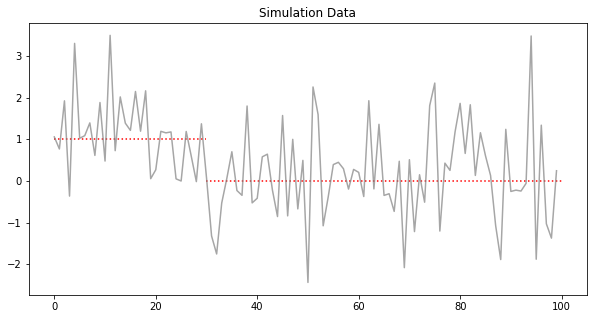
\includegraphics[width=1.0\linewidth]{simulation}
		\caption{Simulation data of $\beta_t$}
		\label{fig:Simulation}
	\end{figure}

	setting the prior as 
	\begin{align*}
	b = 1\;\;&
	b = 1\;\;\\
	c = 1\;\;&
	c = 1\;\;\\
	d = 1\;\;&
	d = 1
	\end{align*}
	and initail values as
	\begin{align*}
	&\gamma_1 = 1 \;\; \eta_1 = 1 \\
	&\gamma_2 = 1 \;\; \eta_2 = 1 \\
	&k=1
	\end{align*}
	Variational distribution is
	\begin{align*}
	q_1^*(\mu_1) &\sim N(1.16, 0.03)\\
	q_2^*(\mu_2) &\sim N(0.13, 0.03)\\
	q_3^*(\tau_1) &\sim Gamma(14.82, 13.61)\\
	q_4^*(\tau_2) \sim Gamma(37.17,86.89)
	\end{align*}
	and $q_5^*$ is
	\begin{figure} [h]
		\centering
		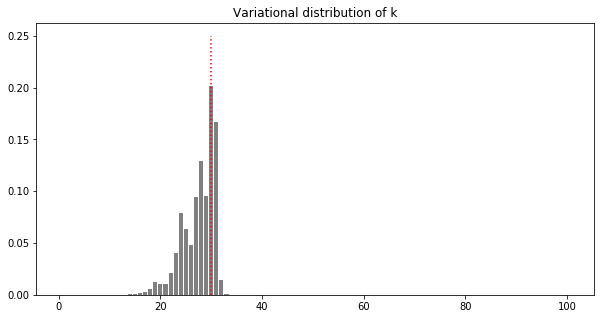
\includegraphics[width=1.0\linewidth]{kproba}
		\caption{Variational distribution of k}
		\label{fig:kproba}
	\end{figure}
	
	
	\begin{align*}
	E_{q_3}^*[k] = 27.65
	\end{align*}


\end{document}